\documentclass[]{book}
\usepackage{lmodern}
\usepackage{amssymb,amsmath}
\usepackage{ifxetex,ifluatex}
\usepackage{fixltx2e} % provides \textsubscript
\ifnum 0\ifxetex 1\fi\ifluatex 1\fi=0 % if pdftex
  \usepackage[T1]{fontenc}
  \usepackage[utf8]{inputenc}
\else % if luatex or xelatex
  \ifxetex
    \usepackage{mathspec}
  \else
    \usepackage{fontspec}
  \fi
  \defaultfontfeatures{Ligatures=TeX,Scale=MatchLowercase}
\fi
% use upquote if available, for straight quotes in verbatim environments
\IfFileExists{upquote.sty}{\usepackage{upquote}}{}
% use microtype if available
\IfFileExists{microtype.sty}{%
\usepackage{microtype}
\UseMicrotypeSet[protrusion]{basicmath} % disable protrusion for tt fonts
}{}
\usepackage[margin=1in]{geometry}
\usepackage{hyperref}
\hypersetup{unicode=true,
            pdftitle={Lines are models},
            pdfauthor={Léo Belzile},
            pdfborder={0 0 0},
            breaklinks=true}
\urlstyle{same}  % don't use monospace font for urls
\usepackage{natbib}
\bibliographystyle{apalike2}
\usepackage{color}
\usepackage{fancyvrb}
\newcommand{\VerbBar}{|}
\newcommand{\VERB}{\Verb[commandchars=\\\{\}]}
\DefineVerbatimEnvironment{Highlighting}{Verbatim}{commandchars=\\\{\}}
% Add ',fontsize=\small' for more characters per line
\usepackage{framed}
\definecolor{shadecolor}{RGB}{248,248,248}
\newenvironment{Shaded}{\begin{snugshade}}{\end{snugshade}}
\newcommand{\AlertTok}[1]{\textcolor[rgb]{0.94,0.16,0.16}{#1}}
\newcommand{\AnnotationTok}[1]{\textcolor[rgb]{0.56,0.35,0.01}{\textbf{\textit{#1}}}}
\newcommand{\AttributeTok}[1]{\textcolor[rgb]{0.77,0.63,0.00}{#1}}
\newcommand{\BaseNTok}[1]{\textcolor[rgb]{0.00,0.00,0.81}{#1}}
\newcommand{\BuiltInTok}[1]{#1}
\newcommand{\CharTok}[1]{\textcolor[rgb]{0.31,0.60,0.02}{#1}}
\newcommand{\CommentTok}[1]{\textcolor[rgb]{0.56,0.35,0.01}{\textit{#1}}}
\newcommand{\CommentVarTok}[1]{\textcolor[rgb]{0.56,0.35,0.01}{\textbf{\textit{#1}}}}
\newcommand{\ConstantTok}[1]{\textcolor[rgb]{0.00,0.00,0.00}{#1}}
\newcommand{\ControlFlowTok}[1]{\textcolor[rgb]{0.13,0.29,0.53}{\textbf{#1}}}
\newcommand{\DataTypeTok}[1]{\textcolor[rgb]{0.13,0.29,0.53}{#1}}
\newcommand{\DecValTok}[1]{\textcolor[rgb]{0.00,0.00,0.81}{#1}}
\newcommand{\DocumentationTok}[1]{\textcolor[rgb]{0.56,0.35,0.01}{\textbf{\textit{#1}}}}
\newcommand{\ErrorTok}[1]{\textcolor[rgb]{0.64,0.00,0.00}{\textbf{#1}}}
\newcommand{\ExtensionTok}[1]{#1}
\newcommand{\FloatTok}[1]{\textcolor[rgb]{0.00,0.00,0.81}{#1}}
\newcommand{\FunctionTok}[1]{\textcolor[rgb]{0.00,0.00,0.00}{#1}}
\newcommand{\ImportTok}[1]{#1}
\newcommand{\InformationTok}[1]{\textcolor[rgb]{0.56,0.35,0.01}{\textbf{\textit{#1}}}}
\newcommand{\KeywordTok}[1]{\textcolor[rgb]{0.13,0.29,0.53}{\textbf{#1}}}
\newcommand{\NormalTok}[1]{#1}
\newcommand{\OperatorTok}[1]{\textcolor[rgb]{0.81,0.36,0.00}{\textbf{#1}}}
\newcommand{\OtherTok}[1]{\textcolor[rgb]{0.56,0.35,0.01}{#1}}
\newcommand{\PreprocessorTok}[1]{\textcolor[rgb]{0.56,0.35,0.01}{\textit{#1}}}
\newcommand{\RegionMarkerTok}[1]{#1}
\newcommand{\SpecialCharTok}[1]{\textcolor[rgb]{0.00,0.00,0.00}{#1}}
\newcommand{\SpecialStringTok}[1]{\textcolor[rgb]{0.31,0.60,0.02}{#1}}
\newcommand{\StringTok}[1]{\textcolor[rgb]{0.31,0.60,0.02}{#1}}
\newcommand{\VariableTok}[1]{\textcolor[rgb]{0.00,0.00,0.00}{#1}}
\newcommand{\VerbatimStringTok}[1]{\textcolor[rgb]{0.31,0.60,0.02}{#1}}
\newcommand{\WarningTok}[1]{\textcolor[rgb]{0.56,0.35,0.01}{\textbf{\textit{#1}}}}
\usepackage{longtable,booktabs}
\usepackage{graphicx,grffile}
\makeatletter
\def\maxwidth{\ifdim\Gin@nat@width>\linewidth\linewidth\else\Gin@nat@width\fi}
\def\maxheight{\ifdim\Gin@nat@height>\textheight\textheight\else\Gin@nat@height\fi}
\makeatother
% Scale images if necessary, so that they will not overflow the page
% margins by default, and it is still possible to overwrite the defaults
% using explicit options in \includegraphics[width, height, ...]{}
\setkeys{Gin}{width=\maxwidth,height=\maxheight,keepaspectratio}
\IfFileExists{parskip.sty}{%
\usepackage{parskip}
}{% else
\setlength{\parindent}{0pt}
\setlength{\parskip}{6pt plus 2pt minus 1pt}
}
\setlength{\emergencystretch}{3em}  % prevent overfull lines
\providecommand{\tightlist}{%
  \setlength{\itemsep}{0pt}\setlength{\parskip}{0pt}}
\setcounter{secnumdepth}{5}
% Redefines (sub)paragraphs to behave more like sections
\ifx\paragraph\undefined\else
\let\oldparagraph\paragraph
\renewcommand{\paragraph}[1]{\oldparagraph{#1}\mbox{}}
\fi
\ifx\subparagraph\undefined\else
\let\oldsubparagraph\subparagraph
\renewcommand{\subparagraph}[1]{\oldsubparagraph{#1}\mbox{}}
\fi

%%% Use protect on footnotes to avoid problems with footnotes in titles
\let\rmarkdownfootnote\footnote%
\def\footnote{\protect\rmarkdownfootnote}

%%% Change title format to be more compact
\usepackage{titling}

% Create subtitle command for use in maketitle
\newcommand{\subtitle}[1]{
  \posttitle{
    \begin{center}\large#1\end{center}
    }
}

\setlength{\droptitle}{-2em}

  \title{Lines are models}
    \pretitle{\vspace{\droptitle}\centering\huge}
  \posttitle{\par}
    \author{Léo Belzile}
    \preauthor{\centering\large\emph}
  \postauthor{\par}
      \predate{\centering\large\emph}
  \postdate{\par}
    \date{Fall 2018, version of 2018-09-17}

\usepackage{booktabs}
\usepackage{amsthm}
\makeatletter
\def\thm@space@setup{%
  \thm@preskip=8pt plus 2pt minus 4pt
  \thm@postskip=\thm@preskip
}
\makeatother

\usepackage{amsthm}
\newtheorem{theorem}{Theorem}[chapter]
\newtheorem{lemma}{Lemma}[chapter]
\theoremstyle{definition}
\newtheorem{definition}{Definition}[chapter]
\newtheorem{corollary}{Corollary}[chapter]
\newtheorem{proposition}{Proposition}[chapter]
\theoremstyle{definition}
\newtheorem{example}{Example}[chapter]
\theoremstyle{definition}
\newtheorem{exercise}{Exercise}[chapter]
\theoremstyle{remark}
\newtheorem*{remark}{Remark}
\newtheorem*{solution}{Solution}
\begin{document}
\maketitle

{
\setcounter{tocdepth}{1}
\tableofcontents
}
\hypertarget{introduction}{%
\chapter*{Introduction}\label{introduction}}
\addcontentsline{toc}{chapter}{Introduction}

We shall use the R programming language througout the course (as it is
free and the most used tool for data analysis, including in statistics
courses at EPFL). Visit \href{https://cran.r-project.org/}{the R-project
website} to download the program. The most popular graphical
cross-platform front-end is
\href{https://www.rstudio.com/products/rstudio/download/}{RStudio
Desktop}.

\textbf{R} is an object-oriented interpreted language. It differs from
usual programming languages in that it is designed for interactive
analyses. Indexing in \textbf{R} starts at one, not zero.

You can find several introductions to \textbf{R} online. Have a look at
the \href{https://cran.r-project.org/manuals.html}{\textbf{R} manuals}
or better at
\href{https://cran.r-project.org/other-docs.html}{contributed manuals}.
A nice official reference is
\href{http://colinfay.me/intro-to-r/index.html}{\emph{An introduction
to} \textbf{RR}}. You may wish to look up the following chapters of the
\textbf{R} language definition
(\href{http://colinfay.me/r-language-definition/evaluation-of-expressions.html}{Evaluation
of expressions} and part of the
\href{http://colinfay.me/r-language-definition/objects.html}{\emph{Objects}
chapter}).

\hypertarget{introduction-projection-matrices}{%
\chapter{Introduction, projection
matrices}\label{introduction-projection-matrices}}

\hypertarget{introduction-1}{%
\section{Introduction}\label{introduction-1}}

I will perform basic manipulations in \textbf{R}; the benefit of the
format used for these notes is that you see the output directly and you
can also copy the code.

\hypertarget{packages}{%
\subsection{Packages}\label{packages}}

The great strength of \textbf{R} comes from its contributed libraries
(called packages), which contain contributed functions and datasets
provided by third parties. Some of these (\texttt{base}, \texttt{stats},
\texttt{graphics}, etc.) are loaded by default whenever you open a
session. To install a package from CRAN, use
\texttt{install.packages("package")}, replacing \texttt{package} by the
package name. Once installed, packages can be loaded using
\texttt{library(package)}; all the functions in \texttt{package} will be
available in the environment. The drawback of this approach is that, if
a function from another package is already present with the same name,
it will be overriden. To palliate to this, you can use the \texttt{::}
syntax to access a single function from an installed package, following
the model \texttt{package::function}.

\hypertarget{basics-of-r}{%
\subsection{\texorpdfstring{Basics of
\textbf{R}}{Basics of R}}\label{basics-of-r}}

\begin{itemize}
\tightlist
\item
  Use \texttt{\textless{}-} to assign to a variable, and \texttt{=} for
  matching arguments inside functions
\item
  Elementary functions include \texttt{sum}, \texttt{min}, \texttt{max},
  \texttt{sqrt}, \texttt{log}, \texttt{exp}, etc.
\item
  Indexing in \textbf{R} starts at 1, \textbf{not} zer.
\item
  \textbf{R} is a vectorized language, so avoid loops as much as
  possible
\item
  integers are obtained by appending \texttt{L} to the number, so
  \texttt{2L} is an integer and \texttt{2} a double.
\end{itemize}

Missing values are indicated by \texttt{NA} or \texttt{NaN}. These are
often found in data sets (where missingness is common) or as a result of
invalid mathematical operations \texttt{log(-2)}. Be careful: \textbf{R}
returns errors much less often than its counterparts, so it is good
practice to check that the output is sensical. There is a special type
for \texttt{NULL} pointers. Logicals are \texttt{TRUE} and
\texttt{FALSE} in capital letters.

\textbf{R} is an object oriented language, and the basic elements in
\textbf{R} are vector. Below are some useful commands for performing
basic manipulation of vectors and matrix operations:

\begin{itemize}
\tightlist
\item
  \texttt{c} creates a vector
\item
  \texttt{cbind} (\texttt{rbind}) binds column (row) vectors
\item
  \texttt{matrix} and \texttt{vector} are constructors
\item
  \texttt{diag} creates a diagonal matrix (by default with ones)
\item
  \texttt{t} is the function for transpose
\item
  \texttt{solve} performs matrix inversion
\item
  \texttt{\%*\%} is matrix multiplication, \texttt{*} is element-wise
  multiplication
\item
  \texttt{crossprod} \texttt{crossprod(A,\ B)} calculates the
  cross-product, \texttt{t(A)\ \%*\%\ B} of two matrices \texttt{A} and
  \texttt{B}
\item
  \texttt{eigen}/\texttt{chol}/\texttt{qr} perform respectively an
  eigendecomposition/Cholesky/QR decomposition of a matrix
\item
  \texttt{rep} creates a vector of duplicates, \texttt{seq} a sequence.
  For integers \(i\), \(j\) with \(i<j\), \texttt{i:j} generates the
  sequence \(i, i+1, \ldots, j-1, j\).
\end{itemize}

Subsetting is fairly intuitive and general; you can use vectors, logical
statements. For example, if \texttt{x} is a vector, then

\begin{itemize}
\tightlist
\item
  \texttt{x{[}2{]}} returns the second element
\item
  \texttt{x{[}-2{]}} returns all but the second element
\item
  \texttt{x{[}1:5{]}} returns the first five elements
\item
  \texttt{x{[}(length(x)\ -\ 5):length(x){]}} returns the last five
  elements
\item
  \texttt{x{[}c(1,\ 2,\ 4){]}} returns the first, second and fourth
  element
\item
  \texttt{x{[}x\ \textgreater{}\ 3{]}} return any element greater than
  3. Possibly an empty vector of length zero!
\item
  \texttt{x{[}\ x\ \textless{}\ -2\ \textbar{}\ x\ \textgreater{}\ 2{]}}
  multiple logical conditions.
\item
  \texttt{which(x\ ==\ max(x))} index of elements satisfying a logical
  condition.
\end{itemize}

For a matrix \texttt{x}, subsetting now involves dimensions row comma
column. Therefore \texttt{{[}1,2{]}} returns the element in the first
row, second column. \texttt{x{[},2{]}} will return all of the rows, but
only the second column. For lists, you can use \texttt{{[}{[}} for
subsetting or the \texttt{\$} signs.

\hypertarget{week1}{%
\section{R-tutorial 1}\label{week1}}

\hypertarget{data-sets}{%
\subsection{Data sets}\label{data-sets}}

We start by loading a dataset of the Old Faithful Geyser of Yellowstone
National park. This is a \texttt{data.frame} object, a matrix whose
columns can be of different types (\texttt{integer}, \texttt{double},
\texttt{logical}, \texttt{character}). To load a package already present
in an \textbf{R} package, use the command \texttt{data} with the name of
the \texttt{package} as a string.

\begin{Shaded}
\begin{Highlighting}[]
\CommentTok{# Load Old faithful dataset}
\KeywordTok{data}\NormalTok{(faithful, }\DataTypeTok{package =} \StringTok{"datasets"}\NormalTok{)}
\CommentTok{# Query the database for documentation}
\NormalTok{?faithful}
\CommentTok{# look at first entries}
\KeywordTok{head}\NormalTok{(faithful)}
\end{Highlighting}
\end{Shaded}

\begin{verbatim}
##   eruptions waiting
## 1     3.600      79
## 2     1.800      54
## 3     3.333      74
## 4     2.283      62
## 5     4.533      85
## 6     2.883      55
\end{verbatim}

\begin{Shaded}
\begin{Highlighting}[]
\KeywordTok{str}\NormalTok{(faithful)}
\end{Highlighting}
\end{Shaded}

\begin{verbatim}
## 'data.frame':    272 obs. of  2 variables:
##  $ eruptions: num  3.6 1.8 3.33 2.28 4.53 ...
##  $ waiting  : num  79 54 74 62 85 55 88 85 51 85 ...
\end{verbatim}

\begin{Shaded}
\begin{Highlighting}[]
\CommentTok{# What kind of object is faithful? }
\KeywordTok{class}\NormalTok{(faithful)}
\end{Highlighting}
\end{Shaded}

\begin{verbatim}
## [1] "data.frame"
\end{verbatim}

Other common classes are \texttt{matrix} and \texttt{list}. The former
has attributes \texttt{dim}, \texttt{ncol} and \texttt{nrow} in addition
to \texttt{length}, which gives the total number of elements. A
\texttt{list} is an unstructured class whose elements are accessed using
double indexing \texttt{{[}{[}\ {]}{]}} and elements are typically
accessed using \texttt{\$} symbol with names. To delete an element from
a list, assign \texttt{NULL} to it. \texttt{data.frame} is a special
type of list where all the elements are vectors of potentially different
type, but of the same length.

\hypertarget{graphics}{%
\subsection{Graphics}\label{graphics}}

The \texttt{faithful} dataset consists of two variables: the regressand
\texttt{waiting} and the regressor \texttt{eruptions}. One could
postulate that the waiting time between eruptions will be smaller if the
eruption time is small, since pressure needs to build up for the
eruption to happen. We can look at the data to see if there is a linear
relationship between the variables.

There are two options: the base graphics package and the package
\texttt{ggplot2}. The syntax for the two options is detailed below.
Always label the axis and include units.

\begin{Shaded}
\begin{Highlighting}[]
\CommentTok{# Scatterplots}
\CommentTok{# Using default R commands}
\KeywordTok{plot}\NormalTok{(waiting }\OperatorTok{~}\StringTok{ }\NormalTok{eruptions, }\DataTypeTok{data =}\NormalTok{ faithful, }
     \DataTypeTok{xlab =} \StringTok{"Eruption time (in min.)"}\NormalTok{, }
     \DataTypeTok{ylab =} \StringTok{"Waiting time between eruptions (in min.)"}\NormalTok{,}
     \DataTypeTok{main =} \StringTok{"Old Faithful Geyser Data"}\NormalTok{)}
\end{Highlighting}
\end{Shaded}

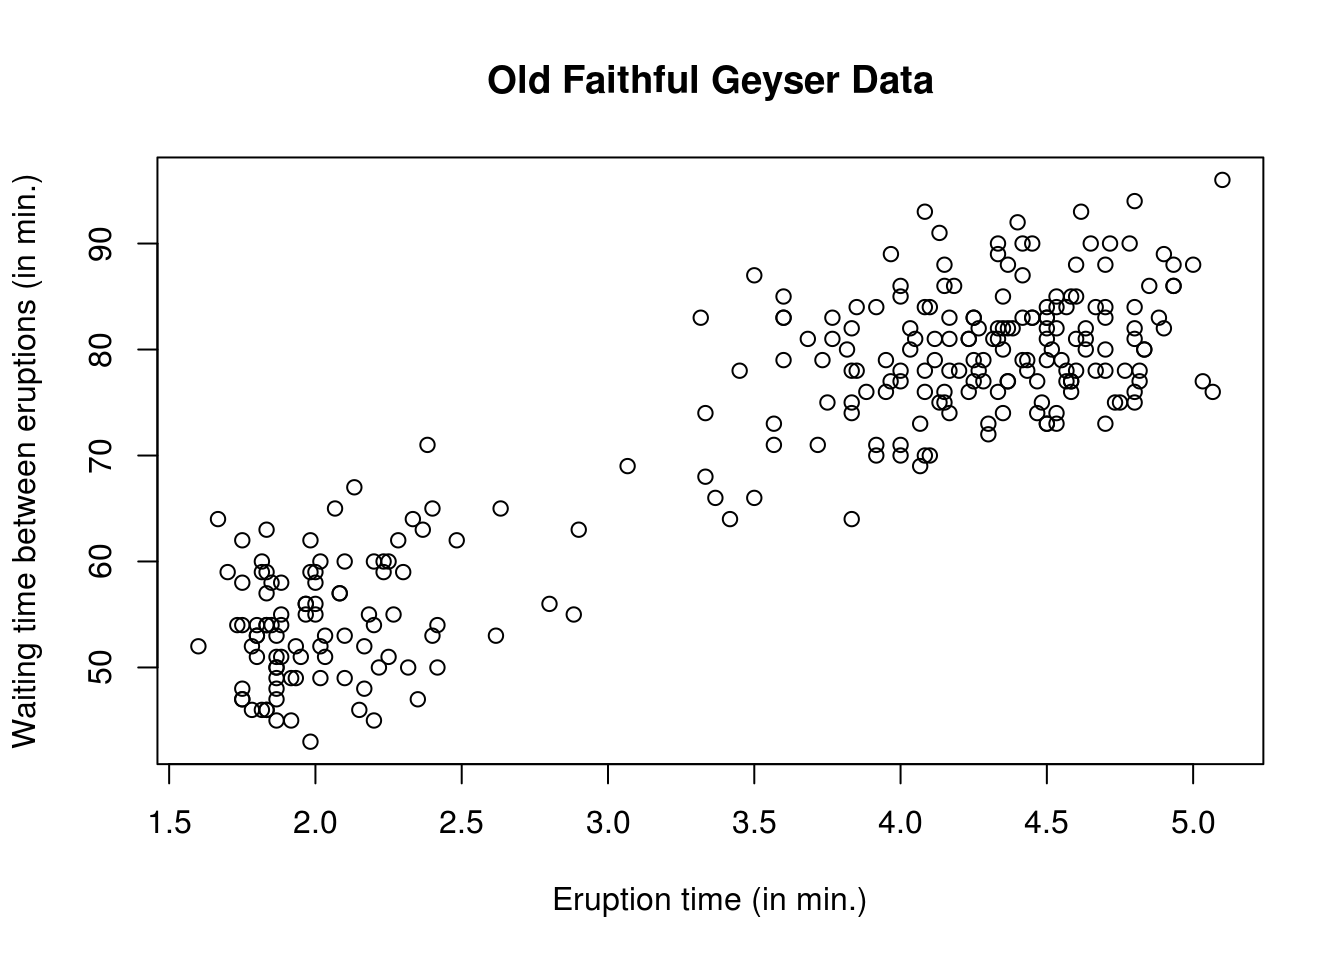
\includegraphics{math341-lines-R-models_files/figure-latex/week1_scatterplot-1.pdf}

\begin{Shaded}
\begin{Highlighting}[]
\CommentTok{#install.packages("ggplot2") #do this once only}
\CommentTok{#using the grammar of graphics (more modular)}
\KeywordTok{library}\NormalTok{(ggplot2)}
\KeywordTok{ggplot}\NormalTok{(}\DataTypeTok{data =}\NormalTok{ faithful, }\KeywordTok{aes}\NormalTok{(}\DataTypeTok{x =}\NormalTok{ eruptions, }\DataTypeTok{y =}\NormalTok{ waiting)) }\OperatorTok{+}\StringTok{ }
\StringTok{  }\KeywordTok{geom_point}\NormalTok{() }\OperatorTok{+}\StringTok{  }
\StringTok{  }\KeywordTok{labs}\NormalTok{(}\DataTypeTok{title =} \StringTok{"Old Faithful Geyser Data"}\NormalTok{, }\DataTypeTok{x =} \StringTok{"Eruption time (in min.)"}\NormalTok{, }\DataTypeTok{y =} \StringTok{"Waiting time between eruptions (in min.)"}\NormalTok{)}
\end{Highlighting}
\end{Shaded}

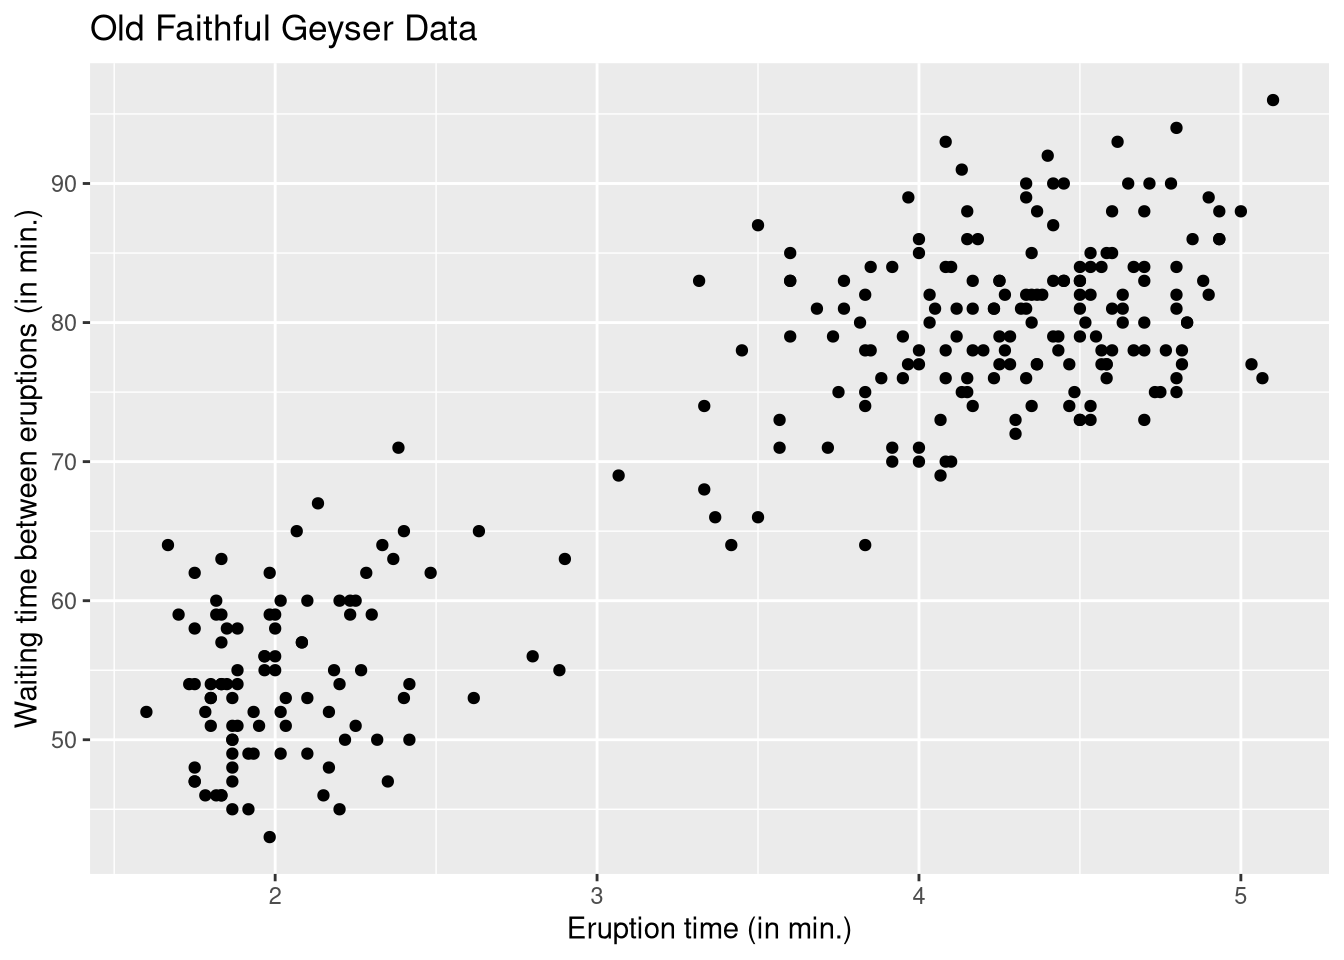
\includegraphics{math341-lines-R-models_files/figure-latex/week1_scatterplot-2.pdf}

A simple linear model of the form
\(y_i = \beta_0 + \beta_1 \mathrm{x}_i + \varepsilon_i\), where
\(\varepsilon_i\) is a noise variable with expectation zero and
\(\mathbf{x} = \mathsf{eruptions}\) and
\(\boldsymbol{y} = \mathsf{waiting}\). We first create a matrix with a
column of \(\mathbf{1}_n\) for the intercept. We bind vectors by column
(\texttt{cbind}) into a matrix, recycling arguments if necessary. Use
\texttt{\textless{}-} to assign values to a variable and \texttt{\$} to
obtain a column of the data frame

\begin{Shaded}
\begin{Highlighting}[]
\CommentTok{## Manipulating matrices}
\NormalTok{n <-}\StringTok{ }\KeywordTok{nrow}\NormalTok{(faithful)}
\NormalTok{p <-}\StringTok{ }\KeywordTok{ncol}\NormalTok{(faithful)}
\NormalTok{y <-}\StringTok{ }\NormalTok{faithful}\OperatorTok{$}\NormalTok{waiting}
\NormalTok{X <-}\StringTok{ }\KeywordTok{cbind}\NormalTok{(}\DecValTok{1}\NormalTok{, faithful}\OperatorTok{$}\NormalTok{eruptions)}
\end{Highlighting}
\end{Shaded}

We can now create an orthogonal projection matrix \texttt{X} onto the
\(\mathsf{span}(\mathbf{X})\). We can verify the properties of
\(\mathbf{H}_{\mathbf{X}}\) numerically using \texttt{all.equal} to
check for equalities.

\hypertarget{projection-matrices}{%
\subsection{Projection matrices}\label{projection-matrices}}

\begin{Shaded}
\begin{Highlighting}[]
\NormalTok{Hx <-}\StringTok{ }\NormalTok{X }\OperatorTok\StringTok{ }\KeywordTok{solve}\NormalTok{(}\KeywordTok{crossprod}\NormalTok{(X)) }\OperatorTok\StringTok{ }\KeywordTok{t}\NormalTok{(X)}
\CommentTok{# Create projection matrix onto complement }
\CommentTok{# `diag(n)` is the n by n identity matrix}
\NormalTok{Mx <-}\StringTok{ }\KeywordTok{diag}\NormalTok{(n) }\OperatorTok{-}\StringTok{ }\NormalTok{Hx}
\CommentTok{#Check that projection leaves X invariant}
\KeywordTok{isTRUE}\NormalTok{(}\KeywordTok{all.equal}\NormalTok{(X, Hx }\OperatorTok\StringTok{ }\NormalTok{X))}
\end{Highlighting}
\end{Shaded}

\begin{verbatim}
## [1] TRUE
\end{verbatim}

\begin{Shaded}
\begin{Highlighting}[]
\CommentTok{#Check that orthogonal projection maps X to zero matrix of dimension (n, p)}
\KeywordTok{isTRUE}\NormalTok{(}\KeywordTok{all.equal}\NormalTok{(}\KeywordTok{matrix}\NormalTok{(}\DecValTok{0}\NormalTok{, }\DataTypeTok{nrow =}\NormalTok{ n, }\DataTypeTok{ncol =}\NormalTok{ p), Mx }\OperatorTok\StringTok{ }\NormalTok{X))}
\end{Highlighting}
\end{Shaded}

\begin{verbatim}
## [1] TRUE
\end{verbatim}

\begin{Shaded}
\begin{Highlighting}[]
\CommentTok{#Check that the matrix Hx is idempotent}
\KeywordTok{isTRUE}\NormalTok{(}\KeywordTok{all.equal}\NormalTok{(Hx }\OperatorTok\StringTok{ }\NormalTok{Hx, Hx))}
\end{Highlighting}
\end{Shaded}

\begin{verbatim}
## [1] TRUE
\end{verbatim}

\begin{Shaded}
\begin{Highlighting}[]
\CommentTok{#Check that the matrix Hx is symmetric}
\KeywordTok{isTRUE}\NormalTok{(}\KeywordTok{all.equal}\NormalTok{(}\KeywordTok{t}\NormalTok{(Hx), Hx))}
\end{Highlighting}
\end{Shaded}

\begin{verbatim}
## [1] TRUE
\end{verbatim}

\begin{Shaded}
\begin{Highlighting}[]
\CommentTok{#Check that only a two eigenvalue are 1 and the rest are zero}
\KeywordTok{isTRUE}\NormalTok{(}\KeywordTok{all.equal}\NormalTok{(}\KeywordTok{eigen}\NormalTok{(Hx, }\DataTypeTok{only.values =} \OtherTok{TRUE}\NormalTok{)}\OperatorTok{$}\NormalTok{values, }\KeywordTok{c}\NormalTok{(}\KeywordTok{rep}\NormalTok{(}\DecValTok{1}\NormalTok{, p), }\KeywordTok{rep}\NormalTok{(}\DecValTok{0}\NormalTok{, n }\OperatorTok{-}\StringTok{ }\NormalTok{p))))}
\end{Highlighting}
\end{Shaded}

\begin{verbatim}
## [1] TRUE
\end{verbatim}

\begin{Shaded}
\begin{Highlighting}[]
\CommentTok{#Check that the matrix has rank p}
\KeywordTok{isTRUE}\NormalTok{(}\KeywordTok{all.equal}\NormalTok{(Matrix}\OperatorTok{::}\KeywordTok{rankMatrix}\NormalTok{(Hx), p, }\DataTypeTok{check.attributes =} \OtherTok{FALSE}\NormalTok{))}
\end{Highlighting}
\end{Shaded}

\begin{verbatim}
## [1] TRUE
\end{verbatim}

\hypertarget{your-turn}{%
\subsection*{Your turn}\label{your-turn}}
\addcontentsline{toc}{subsection}{Your turn}

\begin{itemize}
\tightlist
\item
  Install the \textbf{R} package \texttt{ISLR} and load the dataset
  \texttt{Auto}. Be careful, as \textbf{R} is case-sensitive.
\item
  Query the help file for information about the data set.
\item
  Look at the first lines of \texttt{Auto}
\item
  Create an explanatory variable \texttt{x} with horsepower and mileage
  per gallon as response \texttt{y}.
\item
  Create a scatterplot of \texttt{y} against \texttt{x}. Is there a
  linear relationship between the two variables?
\item
  Append a vector of ones to \texttt{x} and create a projection matrix.
\item
  Check that projection matrix is symmetric and idempotent.
\end{itemize}

\bibliography{book.bib,packages.bib}


\end{document}
